\chapter{Simulations}

This part of Thesis serves as a general description of the \texttt{PyVort} codebase, a new platform to simulate quantum vortices. The code is written in well commented \texttt{Python 3}, arranged in a modular structure. The primary aim of this chapter is to highlight which modules are involved and how they work.
On \href{https://github.com/KuboBahyl/superfluid}{GitHub}, one can find a table of the parameters (user's options) which can be set in the \texttt{config.py} file to run the simulation.

At present, we use infinite boundary conditions. Therefore, only closed-loop vortices can be realized in simulation. However, the codebase is flexible and supports the potential implementation of unclosed loops.

\section{Vortex filament model}

The \texttt{PyVort} code is based on vortex filament (VF) model, a technique pioneerd by Schwarz \cite{schwarz} in the early 1980s. Superfluid vortex filament is represented by a series of mesh points (segments) distributed along the centerline of the filament (\textbf{Figure \ref{example_ring}}). The motion of the whole VF is summed up by the motion of each mesh point.

\begin{figure}[h]
	\centering
	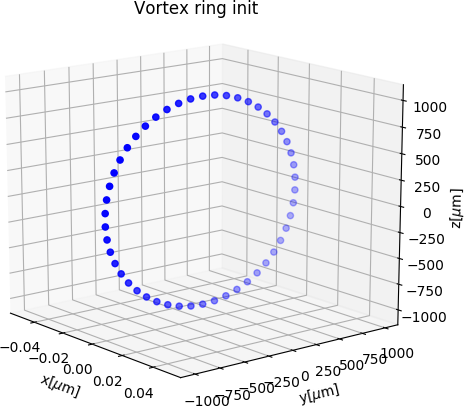
\includegraphics[width=0.5\textwidth]{graphics/simul/ring_init_crop}
	\caption{Visualisation of vortex ring segments right
after their initialisation.}
	\label{example_ring}
\end{figure}

As introduced in \textbf{Theoretical Background} chapter, we define the VF more precisely as a three dimensional curve $\vec{s}(\xi, t)$, where $\xi$ represent an arc-lengths and $t$ the time.
Each segment, indexed as $(i)$ ($i$ is increasing as we move along the VF) is localised by its assigned coordinates $\vec{s}_i$ and direct neighbours indices: \textit{previous} $(i-1)$ and \textit{next} $(i+1)$.\\
This leads to a data structure called as \textit{directed digraph}, which is the array structure we implemented.

Next we define the tangent vector $\vec{s}^{\prime}$, then normal vector $\vec{s}^{\prime\prime}$, and the binormal vector $\vec{s}^{\prime} \times \vec{s}^{\prime\prime}$, as depicted in \textbf{Figure \ref{filament}}, by taking numerical derivatives.
Note $\vec{s}^{\prime} = \text{d}\vec{s} / \text{d}\xi$ and $\vec{s}^{\prime\prime} = \text{d}\vec{s^{\prime}} / \text{d}\xi$.
Numerical derivatives are achieved using \textit{Finite Differences} method, as introduced in next subsection.


\subsection*{Finite differences}

In order to properly calculate the numerical derivatives $\vec{s}^{\prime}$ and $\vec{s}^{\prime\prime}$, belonging to the directed 3D curve, we need to use a sophisticated numerical method. At a particular segment $(i)$ with position $\vec{s}_i$ , we define the distance to the particle in-front $\vec{s}_{i+1}$ as $l_{i} = \vert \vec{s}_{i+1} - \vec{s}_i \vert$ and the distance to the particle behind
$\vec{s}_{i-1}$ as $l_{i-1} = \vert \vec{s}_i - \vec{s}_{i-1} \vert$ (\textbf{Figure \ref{FD}}).
By in-front/behind we refer to the particles next/previous along the filament.

\begin{figure}[h]
	\centering
	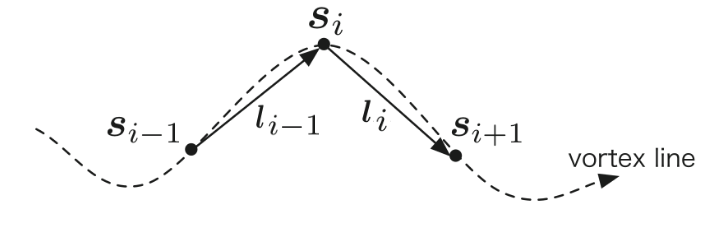
\includegraphics[width=0.8\textwidth]{graphics/simul/finite-diff}
	\caption{Depiction of $i$-th segment vector and its corresponding lengths. Source: \cite{tsubota}}
	\label{FD}
\end{figure}

For accuracy, we approximate all the spatial derivatives $\vec{s}_i^{\prime}$, $\vec{s}_i^{\prime\prime}$ by a
fourth-order finite difference method (FD), which can also account the
varying distances along the vortex filament. With this, the first and second derivatives can be obtained based on coordinates of 2 closest neigbours (on each side).

Using FD theorem, we can construct the approximations by taking the Taylor's series expansions. We can then write:

\begin{equation}
\frac{\text{d}^n\vec{s}_i}{\text{d}\xi^n} \approx
A_i\vec{s}_{i-2} +
B_i\vec{s}_{i-1} +
C_i\vec{s}_{i} +
D_i\vec{s}_{i+1} +
E_i\vec{s}_{i+2}
\hspace{1cm}
\text{for} \,n\in\{1,2\}
\label{FDcoeffs}
\end{equation}

Calculation of coefficients $A, B, C, D, E$ can be done using analytical solution of \textit{Vandermonde matrix} invertion. This invertion can be done also numerically, which is a more scalable way of implementation, however, this method often meets with problems when the Vandermonde matrix becomes singular.
In code, there is implemented both the analytical solution (closed form) and the solution by inverting the Vandermonde matrix. The closed form works for exactly our form of approximation (\ref{FDcoeffs}) and is more described in \cite{FDclosed}, whereas the numerical method works generally for any approximation level.

\subsection*{Biot-Savart discretisation}

We denote the dynamic external sources of velocity fields (which can be set in \texttt{config.py}) as $\vec{v}_{n,ext}(\vec{r}, t)$ and $\vec{v}_{s,ext} (\vec{r}, t)$. The equation of motion for a given segment is then given directly by Schwarz's equation(\ref{schwarz}):

\begin{equation}
\frac{\text{d}\vec{s}_i}{\text{d}t} =
\vec{v}_{s,ext} + \vec{v}_{\text{ind}}^{(i)} + \vec{v}_{\text{drive}}^{(i)}
\end{equation}

The first difficulty in the VF model comes from the calculation of term $\vec{v}_{\text{ind}}$. As we shown previously in (\ref{lia+biot}), this advection term can be split into the LIA part and a Biot-Savart integral:

\begin{align}
\vec{v}_{\text{ind}}^{(i)} =
\vec{v}_{\text{LIA}}^{(i)} + \vec{v}_{\text{BIOT}}^{(i)} =&
\frac{\varkappa}{4\pi} (\vec{s}^{\prime}_i \times \vec{s}^{\prime \prime}_i)
\ln{\Bigg(\frac{2\sqrt{l_{i-1} l_i}}{a}\Bigg)}
\label{LIA}
\\
+& \frac{\varkappa}{4\pi} \int_{\mathcal{L}^{\prime}} \frac{(\vec{r^{\prime}} - \vec{s}_i) \times \text{d}\vec{r^{\prime}}}{\vert \vec{r^{\prime}} - \vec{s}_i \vert^3}\,,
\label{BIOT}
\end{align}

where $l_{i-1}$ and $l_i$ are the arc lengths of the curve between
points $\vec{s}_{i-1}$ and $\vec{s}_i$ and between $\vec{s}_i$ and $\vec{s}_{i+1}$ respectively, and $\mathcal{L}^{\prime}$ is the original vortex line without the two segment lines between $\vec{s}_{i-1}$ and $\vec{s}_{i+1}$.

Using the segment discretisation, the Biot-Savart integral can be rewritten \cite{samuels} into the sum of single-line contributions (\textbf{Figure \ref{element}}) between each $j$-th and $j+1$-th segment (except for the ones attached to the $i$-th point):

\begin{equation}
\vec{v}_{\text{BIOT}}^{(i)} \approx
\frac{\varkappa}{4\pi}
\sum_{j \notin \{i-1, i\}}
\frac{(R_j + R_{j+1}) (\vec{R}_j \times \vec{R}_{j+1})}{R_j R_{j+1} (R_j R_{j+1} + \vec{R}_j \dotprod \vec{R}_{j+1})}\,,
\end{equation}

where $\vec{R}_j = \vec{s}_j - \vec{s}_i$ and $\vec{R}_{j+1} = \vec{s}_{j+1} - \vec{s}_i$ are the relative vectors from the given point.

Note that, if one takes in account the Biot-Savart law for $N$ mesh points, the computational time is proportional to $\mathcal{O}(N^2)$, while, if one uses just the LIA term, it is only $\mathcal{O}(N)$. Numerical simulations based on Biot-Savart are therefore significantly more computationally expensive, even with the speed of today's computers.

\begin{figure}[h]
	\centering
	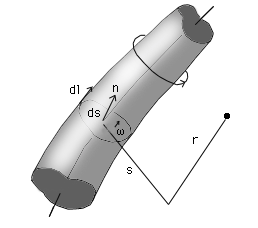
\includegraphics[width=0.5\textwidth]{graphics/simul/biot}
	\caption{An infinitesimal contribution of a $j$-th segment line between two points $\vec{s}_j$ and $\vec{s}_{j+1}$ at a given point $\vec{r}$. Source: \href{http://docs.desktop.aero/appliedaero/potential3d/BiotSavart.html}{Internet}}
	\label{element}
\end{figure}

One way to get around this difficulty is to update the LIA term. In this method we neglect completely the non-local Biot-Savart integral and keep just the local term. This is typically done with a minor adjustments within the log term:

\begin{equation}
\vec{v}_{\text{LIA}}^{*(i)} =
\frac{\varkappa}{4\pi} (\vec{s}^{\prime}_i \times \vec{s}^{\prime \prime}_i)
\ln{\Bigg(\frac{2 R_i}{a}\Bigg)}\,,
\label{LIAnew}
\end{equation}

where $R_i$ is a $i-th$ segment local length scale - may be taken \cite{barenghi} as a local curvature: $R_i = 1 / \vert \vec{s}^{\prime \prime}_i \vert$. Updated LIA approach (\ref{LIAnew}) is a very convenient approximation and works very well for calculating the motion of a single vortex ring.

\section{Implementation}

In code, a system consisting of flow sources and a single vortex ring object is represented using several \texttt{class} structures. These structures are updated after each time step. We will call them as a \textit{state} of the system and it is defined (and initialised) with following properties:

\newpage

\subsection*{Environment class}

\begin{itemize}
	\item \underline{external normal component} - defines an external source of normal component flow
	\item \underline{external normal component} - defines an external source of superfluid component flow
\end{itemize}

\subsection*{Ring class}

This class is initialized only when the purpose of simulation is to collect physical and statistical data about vortex rings.

\begin{itemize}
	\item \underline{center} - an array of ring center coordinates
	\item \underline{radius} - current radius of the ring object
	\item \underline{direction} - a normal vector pointing in a direction toward which the ring is moving
	\item \underline{velocity} - measured velocity of the ring center
\end{itemize}


\subsection*{Vortex class}

\begin{itemize}
	\item \underline{number of active segments} - number of active segments $N$ the vortex ring is composed of
	\item \underline{segments} - an array of all segments, each one with following attributes:
	\begin{itemize}
		\item \underline{activity} - a logical value whether a particular segment should be considered as a part of vortex object
		\item \underline{coordinates} - an array of segment coordinates $\vec{s}_i = [x_i,y_i,z_i]$
		\item \underline{previous/next neighbour} - array localisation indices of the \textit{previous} $(i-1)$ and the \textit{next} $(i+1)$ segment within the context of the directed vortex
		\item \underline{tangent/curvature} - a tangential and normal vectors $\vec{s}^{\prime}_i$ and $\vec{s}^{\prime\prime}_i$

		\item \underline{LIA velocity} - a self-induced velocity $\vec{v}_{\text{LIA}}^{(i)}$ driven by the local curvature.
		\item \underline{BIOT velocity} - a self-induced velocity driven by the farther segment lines of the vortex ring $\vec{v}_{\text{BIOT}}^{(i)}$

		\item \underline{Drive velocity} - a velocity given by the mutual friction force $\vec{v}_{\text{drive}}^{(i)}$
		\item \underline{Full velocity} - the sum of external sources $\vec{v}_{s,ext}$, LIA velocity $\vec{v}_{\text{LIA}}^{(i)}$, BIOT velocity $\vec{v}_{\text{BIOT}}^{(i)}$ and the drive velocity $\vec{v}_{\text{drive}}^{(i)}$, resulting in $\text{d}\vec{s}_i / \text{d}t$
	\end{itemize}
\end{itemize}

All functions that are manipulating with segments' attributes are implemented as Vortex class methods. Before each time stepping, all attributes has to be updated and tested. We used numerical methods already introduced in previous section and tests that are described in next section.

\subsection*{Initialisation}

The proper initialisation of the \textit{state} in the very beginning of simulation requires several physical inputs. This is done in following steps:
\begin{itemize}
	\item[0.] Symbolically, we expect as a \textit{0-th step} the environmental setup of the system - \textit{external sources, temperature, time-step,...}.

	\item[1.] If interested in quantized ring simulation, we expect several ring inputs from user: \textit{center, radius, direction} and \textit{resolution}.
	Resolution parameter is the initial desired distance $\delta$ between each two neigbouring segments. This set of 4 inputs makes an unambiguous ring object, ready for next updates.

	\item[2.] After creation, we initialise neigbour indices (to an $i$-th element in segment array will be assigned $i-1$ index as the \textit{previous} and $i+1$ index as the \textit{next} neighbour index)
	\item[3.] Next we calculate all $\vec{s}^{\prime}$ and $\vec{s}^{\prime\prime}$ using Finite differences method
	\item[4.] Final step is the calculation of all segment velocities using motion equations and their approximative forms.
\end{itemize}

After these four steps, we obtain a fully updated ring object that can be propagated in time.

\newpage

\section{Time evolution}

Now after we defined and ran all the necessary calculations leading to the quantum vortex ring's \textit{state} fulfillment, we can start to propagate it in time.

\begin{figure}[h]
	\centering
	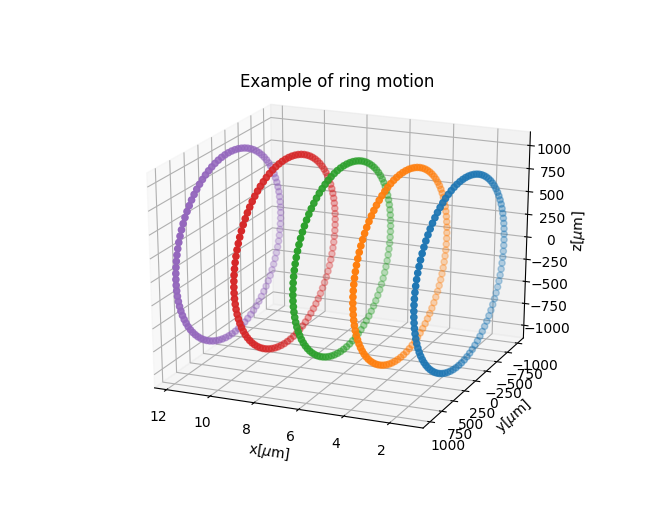
\includegraphics[width=0.8\textwidth]{graphics/simul/time-example}
	\caption{Example of a moving vortex ring}
\end{figure}

\subsection*{Time stepping}

Time evolution is based on an explicit iterative method: the fourth-order Runge-Kutta (RK4) scheme. When we consider the Schwarz's equation $\text{d}\vec{s}_i / \text{d}t \equiv \vec{v}_{\text{full}}^{(i)}$, the stepping algorithm is given as:

\begin{equation}
\vec{s}_{i}(t+\text{d}t) =
\vec{s}_{i}(t) +
\frac{\text{d}t}{6} (\vec{v}_1^{(i)} + 2\vec{v}_2^{(i)} + 2\vec{v}_3^{(i)} + \vec{v}_4^{(i)})\,,
\end{equation}

where $\text{d}t$ is the time step and the velocities $\vec{v}_1^{(i)}, \vec{v}_2^{(i)}, \vec{v}_3^{(i)}, \vec{v}_4^{(i)}$ are the induced velocites of partial steps:

\begin{align}
\vec{v}_1^{(i)} =& \vec{v}_{\text{full}}^{(i)}
(\vec{s}_i, t)\,,
\\
\vec{v}_2^{(i)} =& \vec{v}_{\text{full}}^{(i)}
(\vec{s}_i + \vec{v}_1^{(i)} \text{d}t / 2, t + \text{d}t / 2)\,,
\\
\vec{v}_3^{(i)} =& \vec{v}_{\text{full}}^{(i)}
(\vec{s}_i + \vec{v}_2^{(i)} \text{d}t / 2, t + \text{d}t / 2)\,,
\\
\vec{v}_4^{(i)} =& \vec{v}_{\text{full}}^{(i)}
(\vec{s}_i + \vec{v}_3^{(i)} \text{d}t, t + \text{d}t)
\end{align}

Lower-order schemes such as basic Euler method is also implemented in code, however, not recommended to use. More on this is discussed in Results part of thesis.

The time step $\text{d}t$ is adaptively changing so that the vortex ring cannot move faster than a $1\%$ of its size in a single step. As we will see later in Results, in case of vortex rings with changing radius, the time step $\text{d}t$ has to be iteratively changing after each break of the above rule:

\begin{equation}
\text{d}t \leftarrow \frac{0.01 R}{\vert \vec{v}_c \vert}
\label{adaptive_dt}
\end{equation}

\section{Re-segmentation of vortex}

To obtain the most realistic simulation (to catch effects on any length scale), the natural tendency would be to set the resolution parameter $\delta$ as low as possible. However, the CPU time cost rises rapidly as the number of segments $N$ increases, so there is need to find the best trade-off.

As the distance between neighbouring segments is compressed/enlarged with time due to the physics and numerical inaccuracies, there is need for remove/add segments (\textit{re-segment}) in order to conserve the vortex resolution $\delta$. The closeness (in terms of arclength) of neighbouring segments is therefore measured after each simulation time-step.

We used the simplest re-segmenting criteria - keeping an approximately \textit{uniform distance} between the segments. To ensure this, two boundary conditions were implemented:

\begin{itemize}
	\item[1.] The segment $\vec{s}_{j+1}$ would be removed if:

	\begin{equation}
	\vert \vec{s}_{j+1} - \vec{s}_j \vert < \delta_{\text{min}}\,,
	\end{equation}

	where $\delta_{\text{min}}$ is the minimal distance between two segments. Also, the segment $\vec{s}_j$ would take place somewhere between $\vec{s}_{j-1}$ and $\vec{s}_{j+2}$ so that it will conserve the curvature of vortex. Such result can be obtained using any spline interpolation along nearest neighbours. We worked with 3D local spline using 4 points (in our context they would be $\vec{s}_{j-2}$, $\vec{s}_{j-1}$, $\vec{s}_{j+1}$, $\vec{s}_{j+2}$) and create another 11 interpolated knots.
	Consequently, the new position of $\vec{s}_j$ will sit on the 6-th (the middle one) knot and also.

	\item[2.] In a similar manner, we add a new segment $\vec{s}_{\text{new}}$ between $\vec{s}_{j}$ and $\vec{s}_{j+1}$ if:

	\begin{equation}
	\vert \vec{s}_{j+1} - \vec{s}_j \vert > \delta_{\text{max}}\,,
	\end{equation}

	where $\delta_{\text{max}}$ is the maximal allowed distance between two segments.
\end{itemize}

This method keeps all the distances along the vortex roughly in the range $\delta \in \langle \delta_{\text{min}}, \delta_{\text{max}} \rangle$ and also keeps the geometrical properties.

\subsection*{Real-time tests}

After each time step is done, a few tests are performed, to ensure that vortex itself is behaving according to our expectations. The tests are following:

\begin{itemize}
	\item \underline{Length test} - This test calculates the vortex circumference as $l = \sum_j \vert \vec{s}_j - \vec{s}_{j+1} \vert$ and compare it with the theoretical one $2\pi R$. If the deviation from the theoretical value is too high $>1\%$, the segments are noisy and the process is killed. In case of deviation below $<-1\%$, there is clearly too less segments and resegmentation is called.

	\item \underline{Segmentation test} - Here we check the value $l_j \vert \vec{s}_j - \vec{s}_{j+1} \vert$ for each $j$ and ask whether $l_j \in \langle \delta_{\text{min}}, \delta_{\text{max}} \rangle$. If not, resegmentation is called.

	\item \underline{Smallness test} - If the vortex ring radius would decrease below $R < \delta_{\text{min}}$, the ring is deleted from the simulation.
\end{itemize}

\section{Future implementations}

To make \texttt{Pyvort} a full-fledged quantum vortex simulation, there should be implemented following improvements:

\subsection*{Complexity speedup}

Recent numerical research presented \cite{tree_alg} a new numerical method to compute the evolution of vortex filament. The method is based on an N-body cosmological simulation by Barnes and Hut \cite{barnes}, a \textit{tree algorithm} which considerably speeds up the calculation of Biot-Savart integrals - computational cost scales as $\mathcal{O}(N \log(N))$ rather than $N^2$. Properties of the tree method was tested for a variety of vortex configurations, ranging from simple vortex rings to a counterflow vortex tangle and compared with the LIA approac and the exact Biot-Savart's law.

Implementation of such algorithm is not easy, but definitely worth for the speed-up property.


\subsection*{Re-connection process}

If any lines of two vortices (or even the single one) become very close,
the filaments can reconnect, changing the topology of the system.
Many researchers experimentally reported this is happening and also found analogies with vortex dynamics in the Navier–Stokes equation.

\begin{figure}[h]
	\centering
	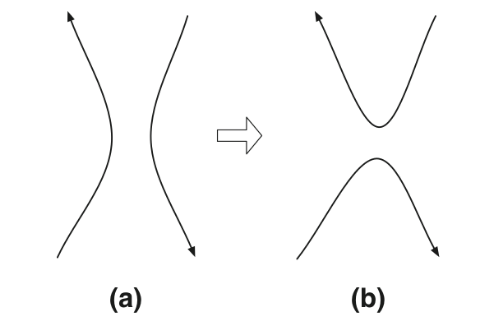
\includegraphics[width=0.6\textwidth]{graphics/simul/reconnection}
	\caption{Reconnection of quantized vortices. \textbf{(a)} Two vortices before reconnection, about to contact each other. \textbf{(b)} The new vortices after reconnection.}
\end{figure}

The VF model itself cannot describe the reconnection process because the vortex core structure is neglected. Hence, some artificial procedures must be introduced to simulate such process. For instance, when two vortices approach within a critical distance $\delta_{\text{min}}$, we will artificially reconnect the vortices.

The main criteria for reconnection is that the total length (this is corresponding with energy) will decrease. Self-reconnections (e.g. caused by a twist of vortex) would be treated in the same way. Since recconection ivolves only antiparallel vortices, one has to check using the inner product whether two vortices could physically reconnect or not.

\subsection*{High-order tests}

Once the code of interacting vortex filaments is developed, the analysis of all that data has to be improved. The simplest measurable quantity is the total lenght of all vortex lines. In a finite volume this would be $L = (1/V) \int \text{d}\xi$ for the vortex line per unit volume.

Of course, there can be defined more complicated metrics, measuring the isotropy of the vortex tangle. One of them is the length of line projected along a given vector $\vec{\hat{r}}$, give as:

\begin{equation}
J(\vec{\hat{r}}) = \frac{1}{VL} \int_{\mathcal{L}} \sqrt{1 - (\vec{s}^{\prime}(\xi) \dotprod \vec{\hat{r}})^2} \text{d}\xi
\end{equation}




\newpage
